\RequirePackage[T1]{fontenc}
\documentclass[journal]{IEEEtran}
\usepackage[round]{natbib}
\usepackage{amsmath,amssymb}
\usepackage{graphicx}
\usepackage{booktabs}
\usepackage{tabularx}
\usepackage{xcolor}
\usepackage{url}
\usepackage[hidelinks]{hyperref}
\hypersetup{pdftitle={HarbourSense: Corrected Public Edition},pdfauthor={Daiyan Khan},pdfsubject={Reproducible synthetic evaluation and system architecture}}
\urlstyle{same}
\def\UrlBreaks{\do\/\do-\do\_\do\.\do\?}
\setlength{\emergencystretch}{2em}
\definecolor{portblue}{RGB}{24,72,95}
\newcommand{\component}[2]{\fcolorbox{portblue}{white}{\parbox[c][1.05cm][c]{#1}{\centering\small #2}}}
\title{Scalable IoT Architecture for Smart Port Asset Tracking and Management: The HarbourSense System}
\author{Daiyan Khan}
\markboth{HarbourSense: Corrected Public Edition, September 2026}{Khan: The HarbourSense System}
\begin{document}
\maketitle

\begin{abstract}
HarbourSense is a software prototype for studying asset tracking, shipment coordination, congestion-aware routing, and crane anomaly handling in a simulated port. A containerized implementation connects Node.js simulators, a Python manager, an Isolation Forest analyzer, MongoDB, an MQTT broker, and a React dashboard. The contribution is an inspectable operational workflow with repeatable scenario inputs, explicit run isolation, acknowledged controls, and recorded outcomes. This public edition replaces earlier unsupported cloud-performance claims with reproducible evidence. An offline evaluation of 2,700 labeled synthetic telemetry samples gives the Isolation Forest 94.86\% precision and 44.58\% recall; a simple range-threshold baseline achieves 100\% precision and 92.58\% recall on the same samples. Both detect all ten injected fault episodes, with median detection delays of 13.5 and 7.5 simulated seconds respectively. In a separate five-seed transport simulation, weighted routing completes an average of 54.2 of 60 shipments within a 600-second horizon, compared with 47.0 for unweighted breadth-first search. Full-stack tests additionally exercise delivery, reset isolation, and recovery from service interruptions. These results support a working demonstration and bounded comparisons, not production scalability, failure prediction, or safety certification. The public website replays captured local runs without operating a public backend.
\end{abstract}

\begin{IEEEkeywords}
Internet of Things, port simulation, MQTT, microservices, anomaly detection, congestion-aware routing, reproducibility.
\end{IEEEkeywords}

\noindent\textit{Edition note---11 September 2026.}
This corrected public edition adapts the original academic write-up to the current implementation and reproducible evaluation. The original source ZIP is preserved separately. Unsupported historical cloud benchmarks and inconsistent performance figures have been removed; the replacement results below identify their inputs, baselines, and limits.

\section{Introduction and Scope}
Port asset management connects several decisions: where an asset is, which shipment it serves, where it should move next, and whether its observed condition requires attention. Tracking alone does not demonstrate that these decisions remain consistent when messages repeat, a service restarts, or a route becomes congested. HarbourSense explores those software coordination problems through a simulated port rather than a deployment on physical port equipment.

The motivation remains the integration of distributed observations with operational decisions. For example, the Port of Rotterdam's Container 42 project collects transport and environmental observations to inform a digital representation of port operations~\citep{rotterdam}. This provides relevant context for telemetry-driven systems, but it does not establish that HarbourSense outperforms an existing port platform. The prototype is deliberately smaller: a fixed port graph, simulated mobile assets and cranes, controlled sensor inputs, and a shipment lifecycle that can be inspected in a dashboard.

The implementation makes three practical contributions. First, it connects telemetry, routing, task assignment, movement, and maintenance handling through real MQTT and MongoDB services. Second, it provides a local demonstration with deterministic scenario inputs and explicit controls for run identity, time, pause, reset, and recovery. Third, it publishes recordings and reproducible evaluation artifacts so a reader can distinguish observed behavior from design intent.

Scalability is an architectural objective in the title, not an experimentally established capacity limit. Separating services creates boundaries that could support independent deployment and tuning. The experiments in this edition do not measure horizontal scaling, cloud resource costs, network savings, production availability, or operation at thousands of devices. No field data, certified safety response, or prospective equipment-failure prediction is claimed.

\section{Design Context and Requirements}
\subsection{From Observation to an Operational Workflow}
RFID, optical identification, positioning systems, and equipment telemetry can provide different observations of a port. HarbourSense does not implement those physical sensing technologies. Its simulators provide software inputs representing asset position, occupancy, and crane condition. The design question is how those inputs affect the next operational action and how that action is acknowledged.

The prototype therefore focuses on five requirements: track current state; complete a shipment through multiple phases; choose routes using the current graph and load inputs; connect anomalous crane telemetry to a maintenance response; and recover from bounded interruptions without presenting stale state as healthy. This scope avoids a claim that one prototype replaces terminal operating systems or supplies a complete digital twin.

\subsection{Messaging and Service Boundaries}
MQTT provides the publish/subscribe transport between producers and consumers. The local demo uses QoS~1, whose protocol semantics permit duplicate delivery~\citep{mqtt}. Consequently, the application must account for repeated events and commands. A broker acknowledgement alone is not proof that a shipment moved, a repair completed, or a database update occurred exactly once.

The implementation separates API request handling from the manager's long-running work. FastAPI supports asynchronous operations~\citep{fastapi}, while independent simulator, sensor, and analyzer processes continue their own message handling. MongoDB stores operational records and demo control state. These are explicit service boundaries; the demo does not demonstrate distributed transactions or unlimited worker replication.

\section{Architecture and Implementation}
\subsection{Two Execution Modes}
Figure~\ref{fig:architecture} distinguishes the local service stack from the public replay. In local mode, eight Compose services provide MongoDB, Mosquitto, the API, the manager, the asset simulator, the sensor simulator, the analyzer, and the dashboard. The broker and database remain on the internal Compose network. The API and dashboard bind to loopback for the supported local workflow.

\begin{figure*}[t]
\centering
\setlength{\tabcolsep}{4pt}
\begin{tabular}{@{}c c c c c@{}}
\component{0.25\textwidth}{Asset and sensor simulators\\Movement and telemetry}
& $\leftrightarrow$ &
\component{0.17\textwidth}{Mosquitto\\MQTT messages}
& $\leftrightarrow$ &
\component{0.25\textwidth}{Manager and analyzer\\Tasks, routes, scores, alerts}
\\[6pt]
\multicolumn{5}{c}{\small Local services persist operational state and observed outcomes in MongoDB.}\\[5pt]
\component{0.25\textwidth}{MongoDB\\Isolated demo-run collections}
& $\leftrightarrow$ &
\component{0.17\textwidth}{FastAPI\\State and controls}
& $\leftrightarrow$ &
\component{0.25\textwidth}{Local React dashboard\\Live service state}
\\[8pt]
\multicolumn{5}{c}{\small Validated recording export $\longrightarrow$ versioned static files $\longrightarrow$ public browser replay}
\end{tabular}
\caption{Current execution boundaries. The upper rows are local services with real MQTT and database processing. The final row is a separate publication path: replay controls operate on captured files in the browser and do not command the local or a public backend.}
\label{fig:architecture}
\end{figure*}

The public site uses a replay adapter over recorded snapshots and events. A recording contains the initial snapshot, subsequent frames, a scenario identifier, simulated duration, and provenance. Playback, speed changes, seeking, and reset operate on that recording. They do not generate new transport outcomes or connect visitors to MongoDB or MQTT. This design fits static hosting: GitHub Pages serves site assets rather than running the Python services~\citep{pages}.

\subsection{Simulation and Shipment Coordination}
The port and sensor simulators execute declared scenario inputs over the existing port fixture. A shipment progresses through arrival, offload, transport, storage, and delivery. The manager and task assigner select work for devices, publish assignments, and handle completion events. Device state includes its current location, route, phase, and assignment identity.

An assignment acknowledgement and a physical movement completion are distinct events. The demo preserves that distinction: terminal shipment outcomes depend on the actual simulator workflow and completion messages. An elapsed timeout is not converted into a fabricated success. The final recording checks also require the relevant device work to be finished and assignments to be cleared.

Maintenance follows the same principle. An analyzer alert can lead to a maintenance task; that task must be assigned, executed, and completed. The dashboard retains the alert history and task outcome so that resolving an alert does not erase the evidence that a fault was detected. Repeated alerts for an ongoing episode are associated with the response rather than implying multiple independent repairs.

\subsection{Congestion-Aware Routing}
The routing component applies a weighted graph search based on the shortest-path approach associated with Dijkstra~\citep{dijkstra}. It is an application of an established algorithm, not a newly established algorithmic contribution. For an edge from $u$ to $v$, the current implementation combines the base weight $w_{uv}$, route congestion $c_{uv}$, current node load $L_v$, a heuristic anticipated load $\widehat{L}_v$, and a grid penalty $g_{uv}$:
\begin{equation}
w'_{uv}=w_{uv}\left(1+c_{uv}+\frac{L_v+\widehat{L}_v}{\tau}\right)+g_{uv}.
\label{eq:cost}
\end{equation}
Here $\tau$ is the configured load normalization threshold. The anticipated load is derived from current movement and alert information; it is not an independently validated learned forecast. The resulting costs can change when the simulated operational state changes. A chosen route is therefore a response to a particular state snapshot and configured cost model.

The live congestion scenario and the offline routing experiment answer different questions. The scenario checks that a real occupancy message reaches the manager and affects an observed route. The offline experiment compares two routing policies under a declared synthetic transport workload; it does not measure the full manager, broker, database, and simulator together.

\subsection{Crane Anomaly Handling}
The analyzer uses the Isolation Forest family of unsupervised anomaly detectors~\citep{iforest}. Its three input features are motor temperature, vibration, and energy use. The model is trained on synthetic normal operating ranges. In the implementation, an exposed anomaly score is the negative of scikit-learn's decision function, so a positive exposed score denotes an anomalous sample under the configured decision rule~\citep{sklearn}.

The analyzer supplies the observed feature values, the model score, and comparisons with the declared training ranges. These comparisons help explain what was unusual in the sample; they are not causal attributions for why equipment failed. A score is also not a probability of failure or an estimate of remaining useful life.

Healthy and anomalous scored telemetry are retained in the demo to support inspection and replay trends. The current path therefore does not forward only alert messages, and no reduction in network traffic is inferred from its architecture. An anomaly event can activate a maintenance response, but the event represents detection of unusual present telemetry rather than prediction of a future physical failure.

\section{Repeatability, Controls, and Recovery}
\subsection{Run Isolation and Logical Time}
Each local demo run has its own identity and database collection namespace. MQTT events carry run identity, and consumers reject events that belong to an old run. Reset creates a fresh namespace and causes workers to rebind. This limits contamination by late work from a prior scenario. Retention and cleanup are bounded to avoid accumulating every historical run indefinitely.

The scenario clock is shared through persisted run state. Start, pause, resume, speed, and reset commands receive acknowledgements. Idempotency identifiers distinguish a retry from a new command. Repeating an acknowledged start command therefore does not silently create a second run.

Pause freezes logical progress and waits for work already in progress to drain before acknowledging the stopped state. Snapshot capture and terminal-state changes share the control lock, preventing a capture from overtaking an acknowledged pause. If an operation cannot drain within the configured bound, the service reports failure with an explicit reset path rather than falsely declaring the run paused.

These mechanisms improve repeatability without claiming that process scheduling and every frame timestamp are bit-for-bit identical. Scenario inputs are deterministic. Outcomes still pass through asynchronous processes, actual messages, and database writes; recordings capture what occurred.

\subsection{Readiness and Interruption Handling}
API reachability is not sufficient readiness. The state endpoint reports freshness and MQTT connection status for the manager, asset simulator, sensor simulator, and analyzer. A stale or disconnected worker is not displayed as healthy merely because a cached snapshot remains available.

The supported local stop command pauses an active scenario before stopping the stack, so a later start can resume its logical state. Arbitrary process termination is a separate failure case. Recovery tests interrupt the API, broker, and MongoDB individually and then verify eventual delivery without duplicate shipments. These checks establish the tested recovery paths; they are not exhaustive proofs for every crash ordering, partition, storage failure, or multi-host deployment.

\subsection{Safe Demonstration Boundary}
Demo controls require explicit demo mode and an allowed local database configuration. Run reset is scoped to owned demo data. No cloud database credentials or device private keys are required for the local demonstration or public replay.

The loopback deployment is not an authenticated public control service. A production deployment would require an independently reviewed authorization model, transport security, secret management, backup and retention policy, resource limits, and operational monitoring. Those requirements are future deployment work, not features implied by the portfolio link.

\section{Evaluation Method}
The corrected results use versioned repository artifacts~\citep{source,evidence}. Table~\ref{tab:evidence} separates the evidence types. All telemetry and workloads are synthetic; no result is a port field trial.

\begin{table*}[t]
\centering
\caption{Evidence types and the conclusions each can support}
\label{tab:evidence}
\small
\begin{tabularx}{\textwidth}{@{}p{0.18\textwidth}p{0.28\textwidth}X@{}}
\toprule
\textbf{Evidence} & \textbf{Execution and inputs} & \textbf{Scope of interpretation}\\
\midrule
Classifier evaluation & Offline scoring of 2,700 labeled synthetic samples & Precision, recall, false alarms, and fault-onset detection delay on the specified generator.\\
Routing evaluation & Offline discrete-event transport simulation, five paired seeds & Policy outcomes under the fixed graph, fleet, workload, bottlenecks, and horizon.\\
Service integration & Real local containers, MQTT messages, MongoDB state, and browser interaction & Functional delivery, command retry behavior, pause/reset invariants, and tested interruption recovery.\\
Public recordings & Captured local scenario snapshots and events & A replayable observation of those runs; playback is not a new experiment or a live service benchmark.\\
\bottomrule
\end{tabularx}
\end{table*}

\subsection{Anomaly Experiment}
The training generator supplies 10,000 synthetic normal samples using seed~42. Its declared feature ranges are 80--90 for motor temperature, 0.1--0.6 for vibration, and 100--120 for energy use. The numerical telemetry scales are demonstration inputs rather than calibrated physical sensor units. The model contamination parameter is 0.01.

Evaluation uses seeds 110, 211, 312, 413, and 514. For each seed, it generates one healthy, one overheating, and one vibration sequence. Each sequence has 180 samples at a one-second simulated interval, giving 15 sequences and 2,700 samples: 1,500 healthy and 1,200 labeled faulty. Fault sequences start their labeled fault period at second~60 and increase the affected features over a 30-second ramp.

The range-threshold baseline flags a sample when any feature lies outside the declared normal range. Both methods receive the same held-out samples. Precision is $TP/(TP+FP)$, recall is $TP/(TP+FN)$, and false-alarm rate is $FP/(FP+TN)$. A separate episode metric measures simulated time from injected fault onset to the first anomaly flag. It must not be interpreted as computer processing time or MQTT/API latency.

\subsection{Routing Experiment}
The routing experiment uses the production weighted route planner and an unweighted breadth-first-search (BFS) baseline inside a separate discrete-event workload. Both strategies receive the same five seeds, 60 shipments per seed, four transport vehicles, and a 600-second simulated horizon. Vehicle start location is E1; origins are A1 or E1 and destinations are B4, D2, or E5. Interarrival gaps are drawn from two to six seconds, base travel is four seconds per hop, and handling takes two seconds.

From second~20 through the declared bottleneck interval ending at second~200, affected traversals incur a 16-second additional hop time. The affected edges are A2--A3, B3--B4, and D1--D2. These are chosen workload conditions, not measured port congestion. Both directions of an edge share a first-in, first-out queue with service capacity for one vehicle at a time. Routes are recomputed at each hop. The offline evaluator leaves predicted node loads empty, so the anticipated-load term used by the production cost model is not active in this comparison. The experiment records completions, unfinished jobs, routing failures, route changes, and delivery times.

Delivery-time summaries include only jobs completed by the horizon. Reported aggregates are means of the five per-seed summaries, with sample standard deviations where stated. They are not pooled latency quantiles, confidence intervals, or estimates of real port throughput. Unfinished jobs must be read alongside delivery time to avoid treating incomplete work as fast service.

\section{Results and Interpretation}
\subsection{Anomaly Detection and Its Baseline}
Table~\ref{tab:anomaly} and Fig.~\ref{fig:anomaly} summarize classification. The Isolation Forest produces 535 true positives, 29 false positives, 665 false negatives, and 1,471 true negatives. The baseline produces 1,111 true positives, no false positives, 89 false negatives, and 1,500 true negatives.

\begin{table}[t]
\centering
\caption{Classification on 2,700 held-out synthetic samples}
\label{tab:anomaly}
\small
\begin{tabular}{@{}lrr@{}}
\toprule
\textbf{Metric} & \textbf{Isolation Forest} & \textbf{Threshold}\\
\midrule
Precision & 94.86\% & 100.00\%\\
Recall & 44.58\% & 92.58\%\\
False-alarm rate & 1.93\% & 0.00\%\\
Fault episodes detected & 10/10 & 10/10\\
Median delay (simulated s) & 13.5 & 7.5\\
\bottomrule
\end{tabular}
\end{table}

\begin{figure*}[t]
\centering
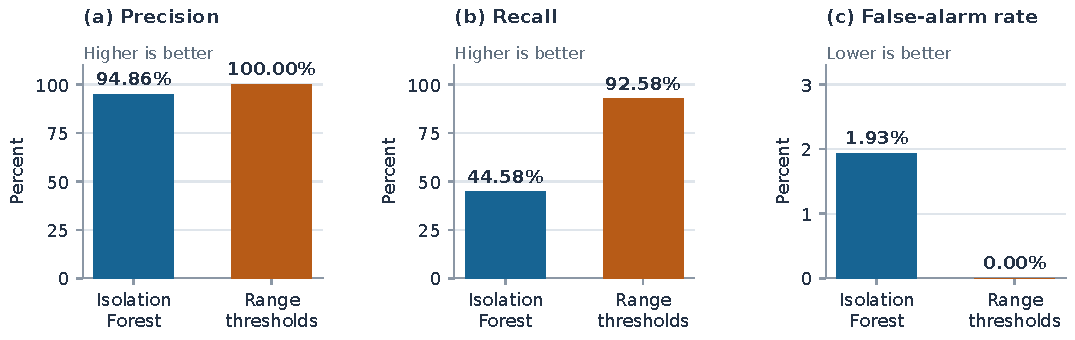
\includegraphics[width=\textwidth]{figures/anomaly-classification.pdf}
\caption{Classification metrics on the shared synthetic evaluation set. The threshold baseline performs better on this generator. Percentages are computed from the committed confusion counts, not from the original report's charts.}
\label{fig:anomaly}
\end{figure*}

The baseline outperforms the model on all three aggregate classification metrics in this workload. This is meaningful even though the model is more complex. The generator defines faults using deviations from the same ranges available to the baseline, making range checks a strong and appropriate reference. A higher model complexity does not by itself establish better operational behavior.

Both methods flag all ten fault episodes at least once, but episode coverage does not imply high per-sample recall. The Isolation Forest can flag an episode and still miss many other labeled faulty samples. Figure~\ref{fig:delay} shows the detection delays; the median is 13.5 simulated seconds for the model and 7.5 for the threshold. These are delays after fault injection, so the experiment does not demonstrate advance warning before a fault.

\begin{figure}[t]
\centering
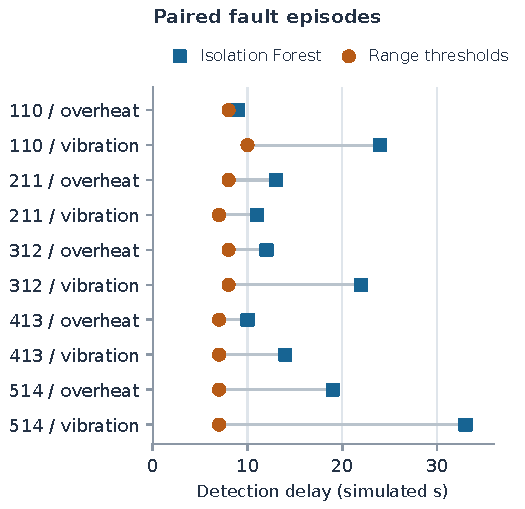
\includegraphics[width=\columnwidth]{figures/anomaly-detection-delay.pdf}
\caption{Fault-onset detection delay for the ten injected fault episodes. Time is measured on the synthetic sequence clock, from onset to the first positive flag. This is not network or inference latency.}
\label{fig:delay}
\end{figure}

The practical conclusion is to retain the threshold baseline and improve the evaluation before arguing for a model-based decision policy. Real telemetry, calibration, operating-condition changes, and costs of false alerts would be needed to assess suitability beyond this generator.

\subsection{Weighted Routing Under the Declared Workload}
The weighted policy completes an average of $54.2\pm3.27$ shipments out of 60 by the horizon, while BFS completes $47.0\pm3.39$ (mean and sample standard deviation across five seeds). The corresponding mean unfinished counts are 5.8 and 13.0. Neither strategy has a route-failure count in these runs. That does not mean every shipment finishes.

\begin{figure*}[t]
\centering
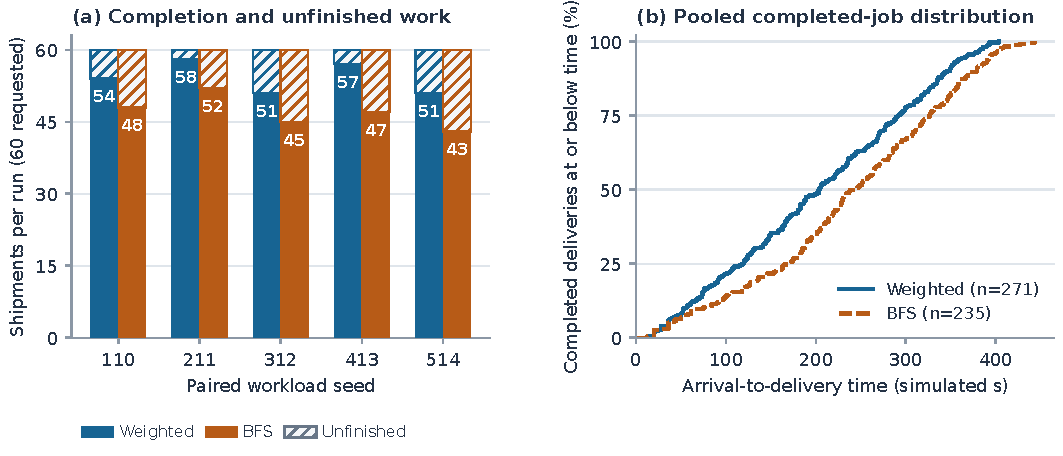
\includegraphics[width=\textwidth]{figures/routing-outcomes.pdf}
\vspace{4pt}
\caption{Routing outcomes for five paired synthetic workloads. Left: completion is counted at the 600-second horizon. Right: the cumulative distribution pools 271 weighted-policy and 235 BFS completed jobs across seeds; unfinished jobs are excluded. The offline workload reuses the weighted planner and does not run the full service stack.}
\label{fig:routing}
\end{figure*}

Mean throughput is 5.42 versus 4.70 completed shipments per simulated minute. The mean of the per-seed median delivery times is 205.3 seconds for weighted routing and 242.1 for BFS, among completed jobs only. The mean of per-seed 95th percentiles is 366.06 versus 390.67 seconds, subject to the same completion condition. Weighted routing records an average of 78.6 route changes per seed; BFS records none.

These outcomes support a benefit for congestion-aware routing under this particular workload. They also expose a trade-off: adapting routes changes operational plans. The experiment does not establish a universal improvement across graphs, bottleneck models, traffic densities, or dispatch policies. Five seeds provide a small repeatability check, not a broad performance characterization.

\subsection{Full-Stack Functional Evidence}
Separate integration checks exercise a real shipment through the local MQTT and MongoDB pipeline, command retries, a stable paused clock and device state, reset during an active run, and recovery after API, broker, and database interruptions. The checked pipeline reaches delivery without duplicate shipments. A clean GitHub-hosted Linux workflow also builds the stack and runs the live browser journey~\citep{ci}.

The recorded normal, congestion, and crane-fault scenarios preserve observed state from local runs. The congestion recording contains an occupancy input and an observed route avoiding its affected node during the injected condition. The crane-fault recording contains scored telemetry, an actual analyzer alert, and a completed maintenance response. All recordings are validated for terminal delivery and cleared assignments before publication.

This is functional evidence of the implemented paths. It is not a cloud benchmark, a measurement of steady-state availability, or proof that no failure ordering can produce a stalled operation. Test durations that include recovery and eventual shipment completion must not be relabeled as reconnect latency.

\section{Reproduction and Public Presentation}
The repository contains scenario specifications, evaluation configurations, raw results, tests, and commands for the local stack~\citep{source,evidence}. The intended local entry point is \texttt{npm run demo}; its readiness checks wait for the API and connected workers. The evaluation scripts rebuild the synthetic results independently of the public replay, while a verification command checks committed result artifacts.

The public website presents three recorded scenarios with playback controls, an event timeline, routing context, crane telemetry, and links to source and evaluation evidence. Recording hashes and provenance support traceability. Visitors can inspect what happened without needing cloud credentials or a local container engine.

Replay time is elapsed simulated time in the recording. It is not current wall-clock telemetry. Similarly, the dashboard's visual health state should be interpreted in its selected data mode: a replay documents a captured run, whereas a local live view depends on current service readiness. Keeping those meanings visible is part of the design, not merely a deployment detail.

\section{Limitations and Future Work}
The most important limitation is external validity. Synthetic feature ranges and injected ramps are easier to label than real equipment data, but they do not capture sensor drift, seasonal conditions, maintenance interventions, or heterogeneous machinery. The threshold's strong result is a reason to question the need for the present model, not a reason to hide the baseline.

The routing workload also simplifies port operations. The graph, fleet, arrival process, travel times, and bottlenecks are fixed by configuration. Completed-only delivery statistics omit jobs still running at the horizon. More seeds, different demand patterns, sensitivity analyses, and explicit uncertainty estimates would make a stronger comparison. Results from this offline workload should remain separate from throughput measurements of the deployed service stack.

The service architecture demonstrates modularity and tested recovery, but it does not yet establish a scale limit or a production operating envelope. Useful next experiments would measure resource use, message volume, end-to-end latency, and recovery behavior under controlled sustained load, with a documented machine configuration and retained raw observations. Until those experiments exist, numerical cloud-savings claims should not be made.

For physical deployment, the task and alert policies would require domain review, calibrated data, and safety boundaries independent of the demonstration software. Authentication, broker security, database backup, and operational ownership would also need explicit design. These are substantial extensions rather than settings that can be inferred from the current portfolio site.

\section{Conclusion}
HarbourSense connects simulated asset observations to routes, shipment tasks, and maintenance responses through an inspectable service pipeline. Its current strengths are a working operational workflow, repeatable inputs, acknowledged controls, run isolation, recovery checks, and an accessible public replay.

The corrected evidence is deliberately bounded. Simple thresholds outperform the current Isolation Forest on the declared synthetic faults, while weighted routing improves completion relative to BFS in the specified offline workload. Real service tests validate selected functional and recovery paths. Together, these results make the prototype useful for explaining architectural decisions and testing future changes, while leaving production performance and equipment-failure prediction as questions for further evidence.

{\raggedright
\renewcommand{\bibfont}{\small}
\bibliographystyle{agsm}
\bibliography{references}
}
\end{document}
